%%p01
En la figura, $AB=BC=CD$. Calcular el valor de ``$\alpha$''.
\begin{figure}[h]
	\begin{tikzpicture}[thick]
		\def\r{4}
		\tkzDefPoint(0,0){A}
		\tkzDefPoint(56:\r){B}
		\tkzDefPointBy[rotation=center B angle 68](A) \tkzGetPoint{C}
		\tkzDefPointBy[rotation=center C angle -124](B) \tkzGetPoint{D}
		\tkzFillAngles[size=5mm,fill=green,opacity=.2](A,B,C B,D,C)
		\tkzMarkAngles[size=5mm,mark=none](A,B,C B,D,C)
		\tkzLabelAngle[pos=.9](A,B,C){$\alpha$}
		\tkzLabelAngle[pos=1.2](B,D,C){$28\dg$}
		\tkzDrawPolygon(A,B,D)
		\tkzDrawSegment(B,C)
		\tkzLabelPoints[below left](A)
		\tkzLabelPoints[above](B)
		\tkzLabelPoints[below](C)
		\tkzLabelPoints[below right](D)
	\end{tikzpicture}
\end{figure}
%%a01
\begin{task}
	* $32\dg$
	* $68\dg$
	* $44\dg$
	* $72\dg$
\end{task}
%%r01
$68\dg$
%%p02
Calcula el valor de ``$x$''.
\begin{figure}[h]
	\begin{tikzpicture}[thick]
		\def\r{3}
		\tkzDefPoints{0/0/O,1.1*\r/0/A}
		\tkzDefPoint(106:\r){B}
		\tkzDefParallelogram(B,O,A) \tkzGetPoint{C}
		\tkzFillAngles[size=4mm,fill=green,opacity=.2](A,O,B O,B,C)
		\tkzMarkAngles[size=4mm,mark=none](A,O,B O,B,C)
		\tkzLabelAngle[shift={(.5,-.4)}](A,O,B){$4x+54\dg$}
		\tkzLabelAngle[shift={(.3,.2)}](O,B,C){$8x-30\dg$}
		\tkzDrawPolygon(B,O,A,C)
	\end{tikzpicture}
\end{figure}
%%a02
\begin{task}
	* $12\dg$
	* $13\dg$
	* $16\dg$
	* $28\dg$
\end{task}
%%r02
$13\dg$
%%p03
En la figura, $\ol{BC}\parallel\ol{AD}$. Calcular ``$\alpha$'' y ``$\beta$''.
\begin{figure}[h]
	\begin{tikzpicture}[thick]
		\def\x{3}
		\tkzDefPoints{-\x/0/A,\x/0/D,-1/\x/O1,1/\x/O2}
		\tkzDefShiftPoint[A](70:1){B1}
		\tkzDefShiftPoint[D](115:1){C1}
		\tkzInterLL(A,B1)(O1,O2) \tkzGetPoint{B}
		\tkzInterLL(D,C1)(O1,O2) \tkzGetPoint{C}
		\tkzFillAngles[size=4mm,fill=green,opacity=.2](D,A,B A,B,C B,C,D C,D,A)
		\tkzMarkAngles[size=4mm,mark=none](D,A,B A,B,C B,C,D C,D,A)
		\tkzLabelAngle(D,A,B){$70\dg$}
		\tkzLabelAngle[pos=.8](A,B,C){$\beta$}
		\tkzLabelAngle[shift={(-.2,.1)}](B,C,D){$2\alpha-5\dg$}
		\tkzLabelAngle[shift={(-.2,-.1)}](C,D,A){$\alpha+5\dg$}
		\tkzDrawPolygon(A,B,C,D)
		\tkzLabelPoints[below left](A)
		\tkzLabelPoints[above left](B)
		\tkzLabelPoints[above right](C)
		\tkzLabelPoints[below right](D)
	\end{tikzpicture}
\end{figure}
%%a03
\begin{mini}[1.4]
	\begin{task}
		* $12\dg$ y $124\dg$
		* $20\dg$ y $36\dg$
		* $70\dg$ y $120\dg$
		* $60\dg$ y $110\dg$
	\end{task}
\end{mini}
%%r03
$60\dg$ y $110\dg$
%%p04
En la figura, calcular ``$x$''.
\begin{figure}[h]
	\begin{tikzpicture}[thick]
		\def\r{3.5}
		\tkzDefPoint(170:\r){A}
		\tkzDefPoint(100:\r){B}
		\tkzDefPoint(10:\r){C}
		\tkzInCenter(A,B,C) \tkzGetPoint{I}
		\tkzDefPointsBy[homothety=center C ratio 1.2](B,I){B1,I1}
		\tkzFillAngles[size=6mm,fill=green,opacity=.2](B,C,I I,C,A C,A,I I,A,B)
		\tkzMarkAngles[size=6mm,mark=|](B,C,I I,C,A)
		\tkzMarkAngles[size=5.4mm,arc=ll,mark=none](C,A,I I,A,B)
		\tkzFillAngles[size=4mm,fill=green,opacity=.2](B1,B,A I1,I,A)
		\tkzMarkAngles[size=4mm,mark=none](B1,B,A I1,I,A)
		\tkzDrawPolygon(A,B,C)
		\tkzDrawSegment(B1,B)
		\tkzDrawSegment(A,I)
		\tkzDrawSegment(I1,C)
		\tkzLabelAngles[pos=1.2](B,C,I I,C,A){$\theta$}
		\tkzLabelAngles(C,A,I I,A,B){$\alpha$}
		\tkzLabelAngle[pos=.7](B1,B,A){$x$}
		\tkzLabelAngle[pos=.9](I1,I,A){$40\dg$}
		\tkzLabelPoints[below left](A)
		\tkzLabelPoints[above right](B)
		\tkzLabelPoints[below right](C)
	\end{tikzpicture}
\end{figure}
%%a04
\begin{task}
	* $60\dg$
	* $80\dg$
	* $75\dg$
	* $120\dg$
\end{task}
%%r04
$80\dg$
%%p05.sp
\begin{mini}
	¿Cuál es el número de lados de aquel polígono regular cuyo ángulo interior es $2$ veces su ángulo exterior?
\end{mini}
%%a05
\begin{enum}
	* $4$
	* $12$
	* $6$
	* $10$
\end{enum}
%%r05
$6$
%%p06.sp
\begin{mini}
	En un polígono regular, el doble del número de diagonales es $5$ veces del número de lados. Luego, la medida de su ángulo interior es:
\end{mini}
%%a06
\begin{task}
	* $120\dg$
	* $135\dg$
	* $180\dg$
	* $105\dg$
\end{task}
%%r06
$135\dg$
%%p07.sp
\begin{mini}
	Si la relación entre el ángulo interior y central de un polígono regular es como $3$ a $2$, hallar el número de lados del polígono.
\end{mini}
%%a07
\begin{task}
	* $3$
	* $2$
	* $5$
	* $4$
\end{task}
%%r07
$5$
%%p08.sp
\begin{mini}
	Calcula la suma de las medidas de los ángulos interiores de:
	\begin{center}
		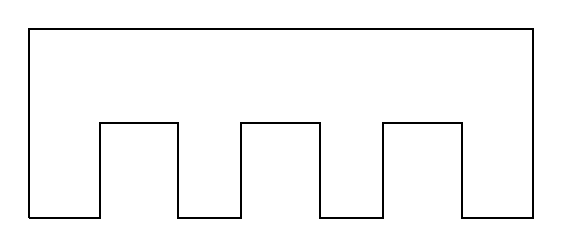
\begin{tikzpicture}[thick]
			\def\x{.8}
			\def\y{.9}
			\def\z{1}
			\def\w{1.2}
			\draw (0,0) -| (\y,\w) -| ++ (\z,-\w) -| ++ (\x,\w) -| ++ (\z,-\w) -| ++ (\x,\w) -| ++ (\z,-\w) -| ++ (\y,2*\w) -| (0,0);
		\end{tikzpicture}
	\end{center}
\end{mini}
%%a08
\begin{task}
	* $2520\dg$
	* $1440\dg$
	* $900\dg$
	* $2880\dg$
\end{task}
%%r08
$2520\dg$
%%p09
Calcular el valor de ``$x$'', en:
\begin{figure}[h]
	\begin{tikzpicture}[thick]
		\def\r{3.5}
		\def\a{9}
		\tkzDefPoint(-170:\r){A}
		\tkzDefPoint(10*\a-10:\r){B}
		\tkzDefPoint(-10:\r){C}
		\tkzDefShiftPoint[A](3*\a:1){I1}
		\tkzDefShiftPoint[C](120+3*\a:1){I2}
		\tkzInterLL(A,I1)(C,I2) \tkzGetPoint{I}
		\tkzFillAngles[size=6mm,fill=green,opacity=.2](A,B,C A,I,C B,C,I I,C,A C,A,I I,A,B)
		\tkzMarkAngles[size=6mm,mark=none](A,B,C A,I,C B,C,I I,C,A C,A,I I,A,B)
		\tkzDrawPolygon(A,B,C)
		\tkzDrawPolySeg(A,I,C)
		\tkzLabelAngle[pos=1](A,B,C){$80\dg$}
		\tkzLabelAngle[pos=.9](A,I,C){$x$}
		\tkzLabelAngle[pos=1.3,rotate=3*\a-60](B,C,I){$2\theta$}
		\tkzLabelAngle[pos=1.2](I,C,A){$3\theta$}
		\tkzLabelAngle[pos=1.2](C,A,I){$3\alpha$}
		\tkzLabelAngle[pos=1.4,rotate=3*\a](I,A,B){$2\alpha$}
	\end{tikzpicture}
\end{figure}
%%a09
\begin{task}
	* $100\dg$
	* $120\dg$
	* $130\dg$
	* $140\dg$
\end{task}
%%r09
$120\dg$
%%p10
\begin{tabular}{c}
	Si $ABCDEF$ es un hexágono regular, calcular ``$x$''. \vspace{5pt} \\
	\begin{tikzpicture}[thick]
		\def\r{2}
		\tkzDefPoints{1.1*\r/0/X,-1.1*\r/0/Y,0/\r/O,0/0/P1}
		\tkzDefRegPolygon[sides=6](O,P1)
		\tkzFillAngles[size=5mm,fill=green,opacity=.2](X,P1,P2 P6,P1,Y)
		\tkzMarkAngles[size=5mm,mark=none](X,P1,P2 P6,P1,Y)
		\tkzDrawPolygon(P1,P...,P6)
		\tkzDrawSegment[<->,>=latex](X,Y)
		\tkzLabelAngles[pos=.9](X,P1,P2 P6,P1,Y){$x$}
		\tkzLabelPoint[below](P1){$A$}
		\tkzLabelPoint[below left](P6){$B$}
		\tkzLabelPoint[above left](P5){$C$}
		\tkzLabelPoint[above](P4){$D$}
		\tkzLabelPoint[above right](P3){$E$}
		\tkzLabelPoint[below right](P2){$F$}
	\end{tikzpicture}
\end{tabular}
%%a10
\begin{task}
	* $30\dg$
	* $15\dg$
	* $20\dg$
	* $45\dg$
\end{task}
%%r10
$30\dg$
%%p11
Calcular ``$x$'' en:
\begin{figure}[h]
	\begin{tikzpicture}[thick]
		\tkzDefPoints{2.8/0/A,0/0/B}
		\tkzDefPointBy[rotation=center B angle 118](A) \tkzGetPoint{C}
		\tkzDefPointBy[rotation=center C angle 108](B) \tkzGetPoint{D1}
		\tkzDefPointBy[homothety=center C ratio 1.3](D1) \tkzGetPoint{D}
		\tkzDefPointBy[rotation=center D angle 98](C) \tkzGetPoint{E1}
		\tkzDefPointBy[rotation=center A angle -128](B) \tkzGetPoint{E2}
		\tkzInterLL(D,E1)(A,E2) \tkzGetPoint{E}
		\tkzFillAngles[size=5mm,fill=green,opacity=.2](E,A,B A,B,C B,C,D C,D,E D,E,A)
		\tkzMarkAngles[size=5mm,mark=none](E,A,B A,B,C B,C,D C,D,E D,E,A)
		\tkzLabelAngle(E,A,B){$x+40\dg$}
		\tkzLabelAngle(A,B,C){$x+30\dg$}
		\tkzLabelAngle[pos=1.3](B,C,D){$x+20\dg$}
		\tkzLabelAngle(C,D,E){$x+10\dg$}
		\tkzLabelAngle[pos=.9](D,E,A){$x$}
		\tkzDrawPolygon(A,B,C,D,E)
	\end{tikzpicture}
\end{figure}
%%a11
\begin{task}
	* $92\dg$
	* $80\dg$
	* $88\dg$
	* $100\dg$
\end{task}
%%r11
$88\dg$
%%p12
Calcula el valor de ``$x$'' del gráfico.
\begin{figure}[h]
	\begin{tikzpicture}[thick]
		\def\r{2.8}
		\tkzDefPoint(-177.5:\r){A}
		\tkzDefPoint(-2.5:\r){C}
		\tkzDefPoints{0/0/D,0/.9*\r/B}
		\tkzFillAngles[size=5mm,fill=green,opacity=.2](D,A,B A,B,C B,C,D)
		\tkzFillAngle[size=3.5mm,fill=green,opacity=.2](C,D,A)
		\tkzMarkAngles[size=5mm,mark=none](D,A,B A,B,C B,C,D)
		\tkzMarkAngle[size=3.5mm,mark=none](C,D,A)
		\tkzDrawPolygon(A,B,C,D)
		\tkzLabelAngles(D,A,B B,C,D){$x$}
		\tkzLabelAngle[pos=.8](A,B,C){$3x$}
		\tkzLabelAngle[pos=.7](C,D,A){$185\dg$}
		\tkzLabelPoints[below left](A)
		\tkzLabelPoints[above](B)
		\tkzLabelPoints[below right](C)
		\tkzLabelPoints[below](D)
	\end{tikzpicture}
\end{figure}
%%a12
\begin{task}
	* $30\dg$
	* $35\dg$
	* $70\dg$
	* $110\dg$
\end{task}
%%r12
$35\dg$
%%p13
Calcula el valor de ``$x$''.
\begin{figure}[h]
	\begin{tikzpicture}[thick]
		\def\r{2.5}
		\tkzDefPoints{0/0/f,.7*\r/-\r/k}
		\tkzDefPointBy[rotation=center k angle -125](f) \tkzGetPoint{j}
		\tkzDefPointBy[rotation=center j angle -115](k) \tkzGetPoint{i1}
		\tkzDefBarycentricPoint(i1=1,j=.3) \tkzGetPoint{i}
		\tkzDefPointBy[rotation=center f angle 110](k) \tkzGetPoint{g1}
		\tkzDefBarycentricPoint(g1=1,f=.1) \tkzGetPoint{g}
		\tkzDefPointBy[rotation=center g angle 135](f) \tkzGetPoint{h1}
		\tkzDefPointBy[rotation=center i angle -140](j) \tkzGetPoint{h2}
		\tkzInterLL(g,h1)(i,h2) \tkzGetPoint{h}
		\def\a{5mm}
		\tkzFillAngles[size=\a,fill=green,opacity=.2](k,f,g f,g,h g,h,i h,i,j i,j,k j,k,f)
		\tkzMarkAngles[size=\a,mark=none](k,f,g f,g,h g,h,i h,i,j i,j,k j,k,f)
		\tkzDrawPolygon(f,g,h,i,j,k)
		\tkzLabelAngle[pos=1.3](k,f,g){$5x-15\dg$}
		\tkzLabelAngle(f,g,h){$5x+10\dg$}
		\tkzLabelAngle[pos=1.1](g,h,i){$3x+20\dg$}
		\tkzLabelAngle[pos=1.3](h,i,j){$5x+15\dg$}
		\tkzLabelAngle(i,j,k){$4x+15\dg$}
		\tkzLabelAngle[pos=.9](j,k,f){$5x$}
		\tkzLabelPoints[left](f)
		\tkzLabelPoints[above left](g)
		\tkzLabelPoints[above right](h)
		\tkzLabelPoints[right](i)
		\tkzLabelPoints[below right](j)
		\tkzLabelPoints[below left](k)
	\end{tikzpicture}
\end{figure}
%%a13
\begin{task}
	* $10\dg$
	* $4\dg$
	* $25\dg$
	* $7\dg$
\end{task}
%%r13
$25\dg$
%%p14
\begin{tabular}{c}
	Si $ABCDE\dots$ es un polígono de $20$ lados, calcular ``$x$''. \vspace{5pt} \\
	\begin{tikzpicture}[thick]
		\def\r{2.5}
		\def\a{1.4}
		\tkzDefPoints{-\a*\r/0/X,\a*\r/0/Y,0/-2.1*\r/O,0/.35*\r/P1}
		\tkzDefRegPolygon[sides=20](O,P1)
		\tkzInterLL(X,Y)(P19,P20) \tkzGetPoint{T1}
		\tkzInterLL(X,Y)(P2,P3) \tkzGetPoint{T2}
		\tkzFillAngles[size=5mm,fill=green,opacity=.2](P20,T1,X Y,T2,P2)
		\tkzMarkAngles[size=5mm,mark=none](P20,T1,X Y,T2,P2)
		\tkzDrawPolySeg(P18,P19,P20,P1,P2,P3,P4)
		\tkzDrawSegment(X,Y)
		\tkzLabelAngles[pos=.9](P20,T1,X Y,T2,P2){$x$}
		\tkzLabelPoint[above left](P3){$A$}
		\tkzLabelPoint[above left](P2){$B$}
		\tkzLabelPoint[above](P1){$C$}
		\tkzLabelPoint[above right](P20){$D$}
		\tkzLabelPoint[above right](P19){$E$}
	\end{tikzpicture}
\end{tabular}
%%a14
\begin{task}
	* $38\dg$
	* $18\dg$
	* $36\dg$
	* $27\dg$
\end{task}
%%r14
$27\dg$
%%p15
Calcula el valor de ``$x$''.
\begin{figure}[h]
	\begin{tikzpicture}[thick]
		\def\r{3}
		\def\a{-3}
		\tkzDefPoint(\a+146:\r){A1}
		\tkzDefPoint(\a+184:\r){B}
		\tkzDefPointOnLine[pos=1.6](B,A1)
		\tkzGetPoint{A}
		\tkzDefPoint(\a-110:\r){C}
		\tkzDefPoint(\a:\r){D1}
		\tkzDefPoint(\a+30:\r){E1}
		\tkzDefParallelogram(A,A1,E1)
		\tkzGetPoint{P1}
		\tkzInterLL(A,P1)(D1,E1)
		\tkzGetPoint{E2}
		\tkzDefPointOnLine[pos=.9](A,E2)
		\tkzGetPoint{E}
		\tkzDefParallelogram(D1,E2,E)
		\tkzGetPoint{P2}
		\tkzInterLL(E,P2)(C,D1)
		\tkzGetPoint{D}
		\tkzFillAngles[size=5mm,fill=green,opacity=.2](B,A,E A,E,D E,D,C D,C,B C,B,A)
		\tkzMarkAngles[size=5mm,mark=none](B,A,E A,E,D E,D,C D,C,B C,B,A)
		\tkzLabelAngles[pos=1.1](B,A,E){$13x-53\dg$}
		\tkzLabelAngle[pos=1.4](C,B,A){$14x-40\dg$}
		\tkzLabelAngle[pos=1](D,C,B){$6x+20\dg$}
		\tkzLabelAngle[pos=1.3](E,D,C){$14x-58\dg$}
		\tkzLabelAngle[pos=1.1](A,E,D){$5x+47\dg$}
		\tkzDrawPolygon(A,B,C,D,E)
		\tkzLabelPoints[above left](A)
		\tkzLabelPoints[left](B)
		\tkzLabelPoints[below](C)
		\tkzLabelPoints[right](D)
		\tkzLabelPoints[above right](E)
	\end{tikzpicture}
\end{figure}
%%a15
\begin{task}
	* $14\dg$
	* $13\dg$
	* $12\dg$
	* $15\dg$
\end{task}
%%r15
$12\dg$
